\documentclass{physlab}
\usepackage{ctable}
\usepackage{tabu}

%\newenvironment{bottompar}{\par\vspace*{\fill}}{\clearpage}

\begin{document}
	\begin{titlepage}
\center % Center everything on the page
 
%----------------------------------------------------------------------------------------
%	HEADING SECTIONS
%----------------------------------------------------------------------------------------

\textsc{\LARGE Московский\\[-0.2cm]Физико-Технический Институт\\[0.1cm]\large (государственный университет)}\\[1.5cm] % Name of your university/college
\textsc{\Large Кафедра общей физики}\\[0.1cm] % Major heading such as course name
\textsc{\large Лабораторная работа № 3.1.1}\\[0.5cm] % Minor heading such as course title

%----------------------------------------------------------------------------------------
%	TITLE SECTION
%----------------------------------------------------------------------------------------

\HRule
\\[0.6cm]
{ \huge \bfseries Магнитометр}
\\[0.3cm] % Title of your document
\HRule
\\[1.5cm]


 
%----------------------------------------------------------------------------------------
%	AUTHOR SECTION
%----------------------------------------------------------------------------------------

\begin{minipage}[t]{0.48\textwidth}
	\begin{flushleft} \large
		\textsf{Студент}\bigskip
		
		\tline{(имя)}{30mm} \tline{(фамилия)}{45mm} \\[5mm]
		\underline{\hspace{30mm}} группа
	\end{flushleft}
\end{minipage}
\hfill
\begin{minipage}[t]{0.48\textwidth}
	\begin{flushright} \large
		\textsf{Преподаватель}\bigskip
		
		\tline{(имя)}{30mm} \tline{(отчество)}{45mm} \\[5mm]
		\tline{(фамилия)}{45mm}
	\end{flushright}
\end{minipage}

\begin{bottompar}
	\begin{center}
		
\includegraphics[width = 80 mm]{logo.jpg}
	\end{center}
	\tline{(дата)}{80mm}

\end{bottompar}
\vfill % Fill the rest of the page with whitespace

\end{titlepage}

\paragraph{Цель работы:} Измерение подвижности и концентрации носителей заряда в полупроводниках.

\paragraph{В работе используются:} \textit{электромагнит с источником питания, амперметр, миллиамперметр, милливеберметр, реостат, цифровой вольтметр, источник питания, образцы легированного германия.}


\section{Теоретическая часть}

\paragraph{Дырки}

Эффект Холла, возникающий в проводниках, происходит из-за наличия некоторого количества свободных электронов в зоне проводимости и такого же количества дырок в валентной зоне. Чтобы понять причину образования дырок, нужно рассмотреть дырочную проводимость.


Дырочную проводимость можно объяснить при помощи следующей аналогии: если представить ряд людей, сидящих в аудитории, где нет запасных стульев. Когда кто-нибудь из середины ряда хочет уйти, он      перелезает через спинку стула в пустой ряд и уходит. Здесь пустой ряд — аналог зоны проводимости, а ушедшего человека можно сравнить со свободным электроном.
Теперь представим, что ещё кто-то пришёл и хочет сесть. Из пустого ряда плохо видно, поэтому там он не садится. Вместо этого человек, сидящий возле свободного стула, пересаживается на него, вслед за ним это повторяют и все его соседи. Таким образом, пустое место как бы двигается к краю ряда. Когда это место окажется рядом с новым зрителем, он сможет сесть.
В этом процессе каждый сидящий передвинулся вдоль ряда. Если бы зрители обладали отрицательным зарядом, такое движение было бы  \textit{электрической проводимостью}. Если вдобавок стулья заряжены положительно, то ненулевым суммарным зарядом будет обладать только свободное место. Это простая модель, показывающая как работает \textit{дырочная проводимость}. Однако на самом деле, из-за свойств кристаллической решётки, дырка не локализована в определённом месте, как описано выше, а размазана по области размером во много сотен элементарных ячеек.\\[-10mm]
\paragraph{Эффект Холла} 
Магнитного поле в проводнике действует на свободные электроны в зоне проводимости, поэтому между гранями наблюдается добавочная разность потенциалов, связанная с силой Лоренца.

\begin {figure}[H]
	\begin{center}
		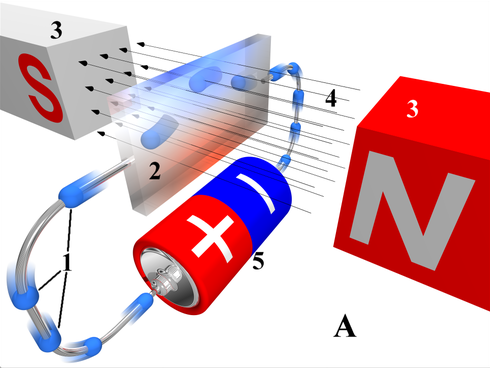
\includegraphics[width = 0.35 \textwidth]{hall_effect}
		\caption{Пример действия эффекта Холла на свободные заряды}
	\end{center}
\end {figure}



$$\boldsymbol{F_\text{Л}}  = -e \boldsymbol{E} - e \langle \boldsymbol{\upsilon} \rangle \times \boldsymbol{B},$$
где $e$ - абсолютная величина заряда электрона, $\boldsymbol{B}$ - индукция магнитного поля, $\boldsymbol{E}$ - напряженность электрического поля, $ \langle \boldsymbol{\upsilon} \rangle$ - средняя скорость заряда.

Из этого выражения получим разность потенциалов между двумя гранями:

\begin{equation}
U = -E_zl = - | \langle \upsilon \rangle | B l
\label{eq:pot_dif}
\end{equation}

С этой возникшей разностью потенциалов и связан Эффект Холла.

Далее, если выразить ток:
$$ I = ne |\langle \upsilon \rangle |  l a$$
И совместить его с \eqref{eq:pot_dif}, получим ЭДС Холла:

\begin{equation}
\mathscr{E}_x = U = - \dfrac{IB}{nea} = -R_x \cdot \dfrac{IB}{a},
\label{eq:hall}
\end{equation}

где $R_x = \dfrac{1}{ne}$ называется \textit{постоянной Холла.}

\section{Установка и параметры измерения}

\begin{wrapfigure}{L}{0.7 \textwidth}
\centering
    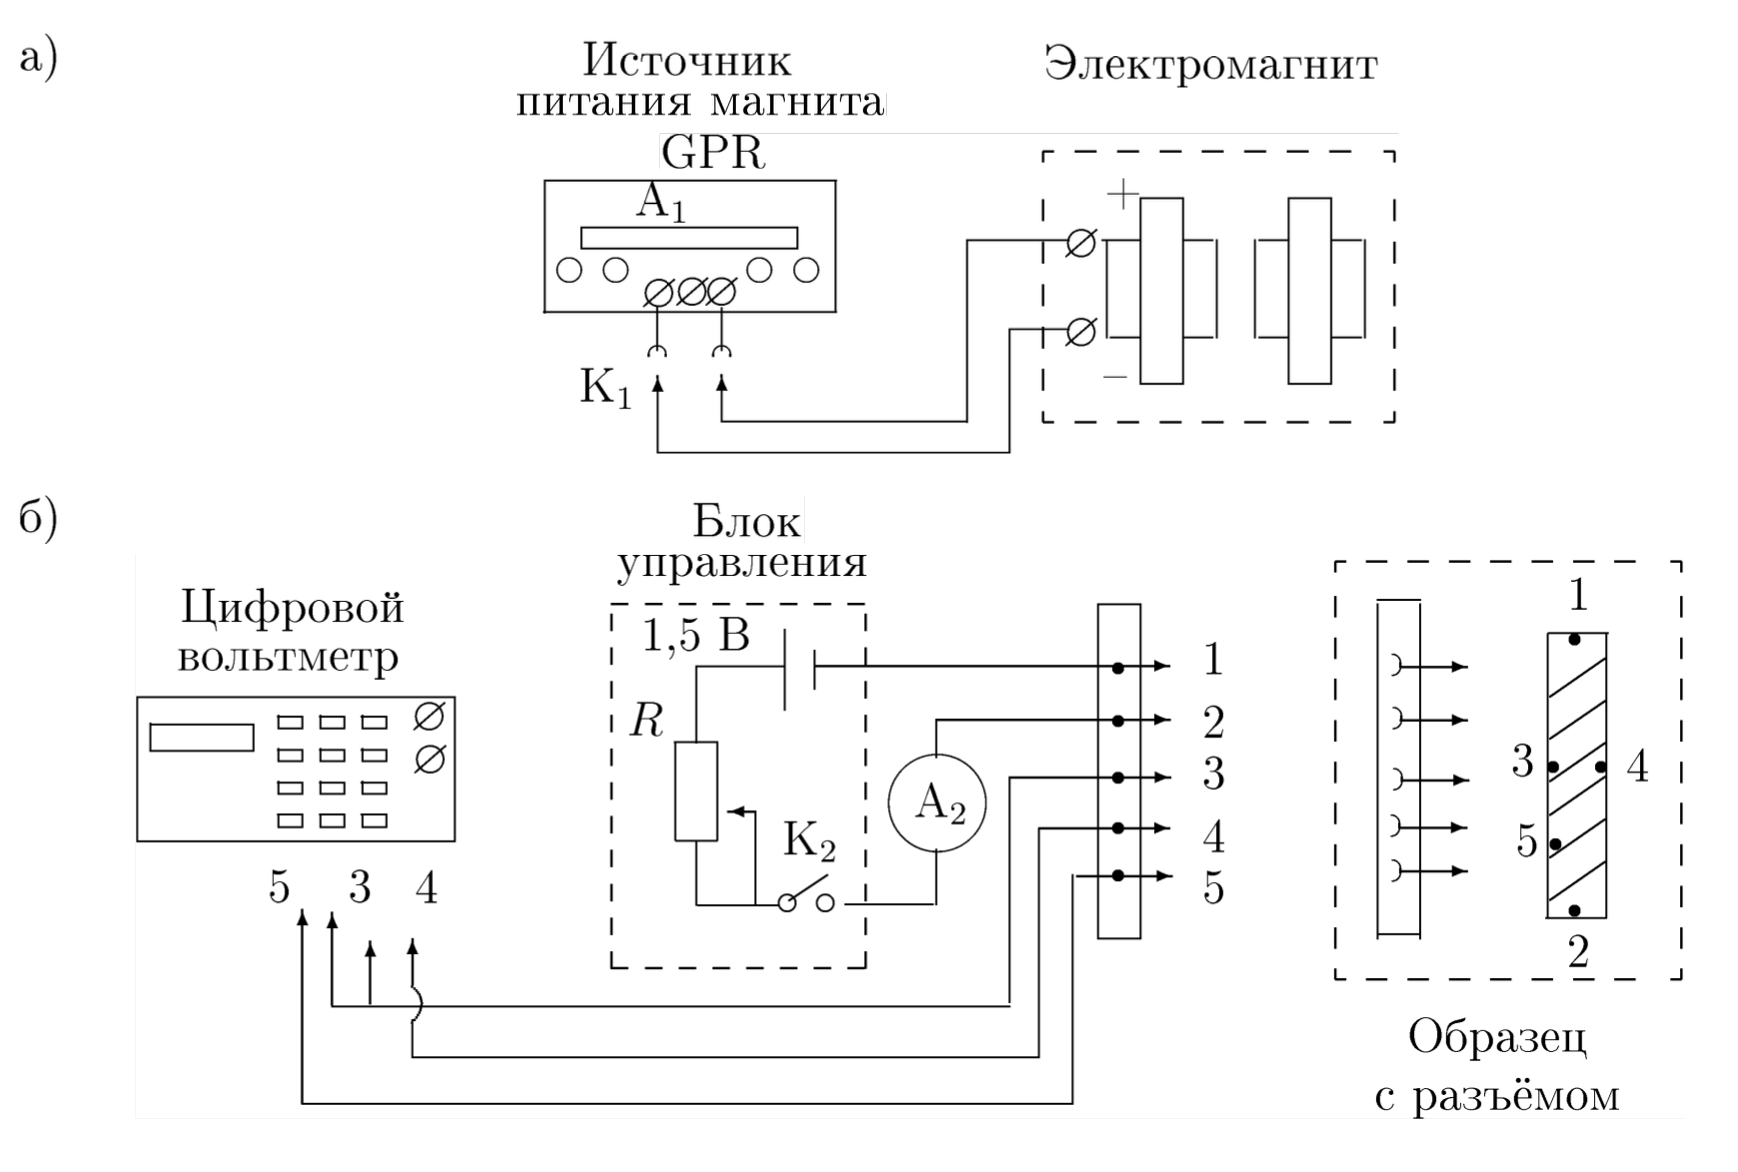
\includegraphics[width = 0.7 \textwidth]{scheme.png}
\caption{Схема установки для измерения эффекта Холла в полупроводниках}
\end{wrapfigure} 

$$\text{Параметры установки:}$$
\begin{align*}
a &= \val \\[1ex]
L_{35} &= \val \\[1ex]
l &= \val
\end{align*}
\vspace{5.7 cm}

В нашей установке вдоль длинной стороны образца будет течь ток, величина которого регулируется реостатом $R_2$. Так как он помещен в электромагнит, между точками \textit{3 и 4} будет возникать разность потенциалов $U_{34}$, которую мы будем измерять. 

Однако между точками \textit{3 и 4} будет возникать некоторое дополнительное падение напряжения $U_{0}$, так как эти точки оказываются не на одной эквипотенциали. Исключить это влияние можно с помощью изменения направления магнитного поля: в одном случае $U_{34} = U_{0} - \mathscr{E}_x $, в другом  $U_{34} = \mathscr{E}_x - U_0$. Тогда с помощью полуразности избавимся от $U_{0}$ в наших измерениях. 

\begin{figure}[H]
	\begin{center}
		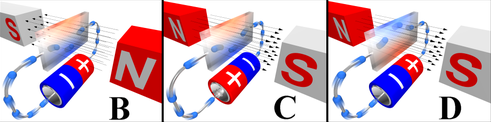
\includegraphics[width = 0.6 \textwidth]{hall_dif}
		\caption{Эффект Холла при различных направлениях магнитного поля и тока через образец}
	\end{center}
\end{figure}


\section{Обработка результатов}

\paragraph{Калибровка установки}
Во время проведения работы мы сняли зависимость магнитного потока $\varPhi$ от силы тока $I$, также нам известно, что $\varPhi=BSN$, где $SN=75\text{ см}^2\cdot\text{вит}$.

\begin{table}[H]
\centering
\caption{Данные для калибровки установки}
\resizebox{\linewidth}{!}{
\begin{tabular}{|c|c|c|c|c|c|c|c|c|}
\hline
$I, \; \m \A$ & \val    & \val   & \val & \val   & \val   & \val & \val     & \val   \\ \hline
$\varPhi, \; \m \Wb$ & \val & \val & \val & \val & \val & \val & \val & \val  \\ \hline
$B, \; \T$ & \val & \val & \val &\val & \val & \val& \val & \val \\ \hline
\end{tabular}
}
\label{calibrate}
\end{table}

\begin{figure}[b!]\centering
	\label{graph1}
	
\includegraphics[width=.65\tw]{foo}
			\caption{Калибровка установки}
	\end {figure}
С помощью МНК вычислим зависимость, $B = \val$

\begin{table}[H]
	\centering
	\caption{Зависимость ЭДС Холла от магнитного поля}
	\resizebox{\linewidth}{!}{
	\begin{tabu}to 1.05\textwidth{|c|c|c|X[c]|X[c]|X[c]|X[c]|X[c]|X[c]|X[c]|X[c]|}
		\hline
		\multirow{2}{*}{$I, \text{ мА}$} & \multirow{2}{*}{$U_0, \text{ мВ}$} & $I_M, \text{ мА}$                                                      &     &    &     &     &     &   &     &     \\ \cline{3-11}
		&                                    & $B, \text{ Тл}$                                                        &  &   &   &   &   &  &   &   \\ \hline
		\multirow{2}{*}{}             & \multirow{2}{*}{}              & $U, \text{мВ}$                                                         &   &  & &  &  & & &  \\ \cline{3-11} 
		&                                    & \begin{tabular}[c]{@{}c@{}}$\mathscr{E}_x,$  $ \text{мВ}$\end{tabular} & &  & &  &  &  &  & \\ \hline
		\multirow{2}{*}{}             & \multirow{2}{*}{}              & $U, \text{мВ}$                                                         &   &  & &  &  & & &  \\ \cline{3-11} 
		&                                    & \begin{tabular}[c]{@{}c@{}}$\mathscr{E}_x,$  $ \text{мВ}$\end{tabular} & &  & &  &  &  &  & \\ \hline	
		\multirow{2}{*}{}             & \multirow{2}{*}{}              & $U, \text{мВ}$                                                         &   &  & &  &  & & &  \\ \cline{3-11} 
		&                                    & \begin{tabular}[c]{@{}c@{}}$\mathscr{E}_x,$  $ \text{мВ}$\end{tabular} & &  & &  &  &  &  & \\ \hline
		\multirow{2}{*}{}             & \multirow{2}{*}{}              & $U, \text{мВ}$                                                         &   &  & &  &  & & &  \\ \cline{3-11} 
		&                                    & \begin{tabular}[c]{@{}c@{}}$\mathscr{E}_x,$  $ \text{мВ}$\end{tabular} & &  & &  &  &  &  & \\ \hline	
		\multirow{2}{*}{}             & \multirow{2}{*}{}              & $U, \text{мВ}$                                                         &   &  & &  &  & & &  \\ \cline{3-11} 
		&                                    & \begin{tabular}[c]{@{}c@{}}$\mathscr{E}_x,$  $ \text{мВ}$\end{tabular} & &  & &  &  &  &  & \\ \hline
		\multirow{2}{*}{}             & \multirow{2}{*}{}              & $U, \text{мВ}$                                                         &   &  & &  &  & & &  \\ \cline{3-11} 
		&                                    & \begin{tabular}[c]{@{}c@{}}$\mathscr{E}_x,$  $ \text{мВ}$\end{tabular} & &  & &  &  &  &  & \\ \hline	
		\multirow{2}{*}{}             & \multirow{2}{*}{}              & $U, \text{мВ}$                                                         &   &  & &  &  & & &  \\ \cline{3-11} 
		&                                    & \begin{tabular}[c]{@{}c@{}}$\mathscr{E}_x,$  $ \text{мВ}$\end{tabular} & &  & &  &  &  &  & \\ \hline
		\multirow{2}{*}{}             & \multirow{2}{*}{}              & $U, \text{мВ}$                                                         &   &  & &  &  & & &  \\ \cline{3-11} 
		&                                    & \begin{tabular}[c]{@{}c@{}}$\mathscr{E}_x,$  $ \text{мВ}$\end{tabular} & &  & &  &  &  &  & \\ \hline	
		\multirow{2}{*}{}             & \multirow{2}{*}{}              & $U, \text{мВ}$                                                         &   &  & &  &  & & &  \\ \cline{3-11} 
		&                                    & \begin{tabular}[c]{@{}c@{}}$\mathscr{E}_x,$  $ \text{мВ}$\end{tabular} & &  & &  &  &  &  & \\ \hline	
	\end{tabu}
}
\end{table}

Проанализируем полученные данные с помощью МНК. Отобразим их в таблице~\ref{tbl:I(k)}:

\begin{table}[H]
	\centering
	\caption{Зависимость углового коэффициента от силы тока}
	\label{tbl:I(k)}
	\begin{tabu}{|c|X[c]|X[c] |X[c]| X[c]| X[c]| X[c]| X[c]| X[c]|}
		\hline
		$I, \text{ мА}$                                           & \val    &    &     &    &     &     &    &    \\ \hline
		$k,\,\text{мВ}\cdot\text{Тл}\slash\text{мА}$          & & & & & & & &\\ \hline
		$\sigma_k\,\text{мВ}\cdot\text{Тл}\slash\text{мА}$ & & & & & & & &  \\ \hline
		$\sigma_I, \text{ мА}$                                 & \multicolumn{8}{c|}{\val}                                             \\\hline
	\end{tabu}
\end{table}
Также изобразим эти данные на графике (рис.~\ref{img:k(I)}). Опять же с помощью МНК получаем, что
\[K = \val\]

Из формулы \eqref{eq:hall} посчитаем постоянную Холла:
\[ R_x = \val \]

\begin {figure}[H]
\centering
	
\includegraphics[width = 0.65 \textwidth]{foo}
\caption{График зависимости $\mathscr{E}_x = f(B)$ для разных $I$}
\end {figure}
	
\begin {figure}[H]
\centering
    
\includegraphics[width = 0.65 \textwidth]{foo}
\caption{График зависимости углового коэффициента от силы тока}
\label{img:k(I)}
\end {figure}

Определим концентрацию носителей заряда: $n = \val$
	
Вычислим удельную проводимость материала с помощью $U_{35}=\val$:
\[\sigma=\val\]

Рассчитаем подвижность электрона:
\begin{align*}
b &= \val \\[1ex]
\Delta b &=\val
\end{align*}


\section{Вывод}

~\\[-1ex]\hrule~\\[1ex]\hrule~\\[1ex]\hrule~\\[1ex]\hrule~\\[1ex]\hrule~\\[1ex]\hrule~\\[1ex]\hrule~\\[1ex]\hrule
\end{document}
